This section outlines the architectural strategy for the flow of the RV8 work cell system, defining the top-level logical view of the design. The system is structured into three distinct layers: Input, Processing, and Output. Each of these layers serves a specific and vital function within the system, enabling the robot to perform fixed tasks based on the program. This section includes a high-level block diagram that visually illustrates the relationships and interactions between these layers, providing a comprehensive overview of the system's architecture.

\begin{figure}[h!]
	\centering
 	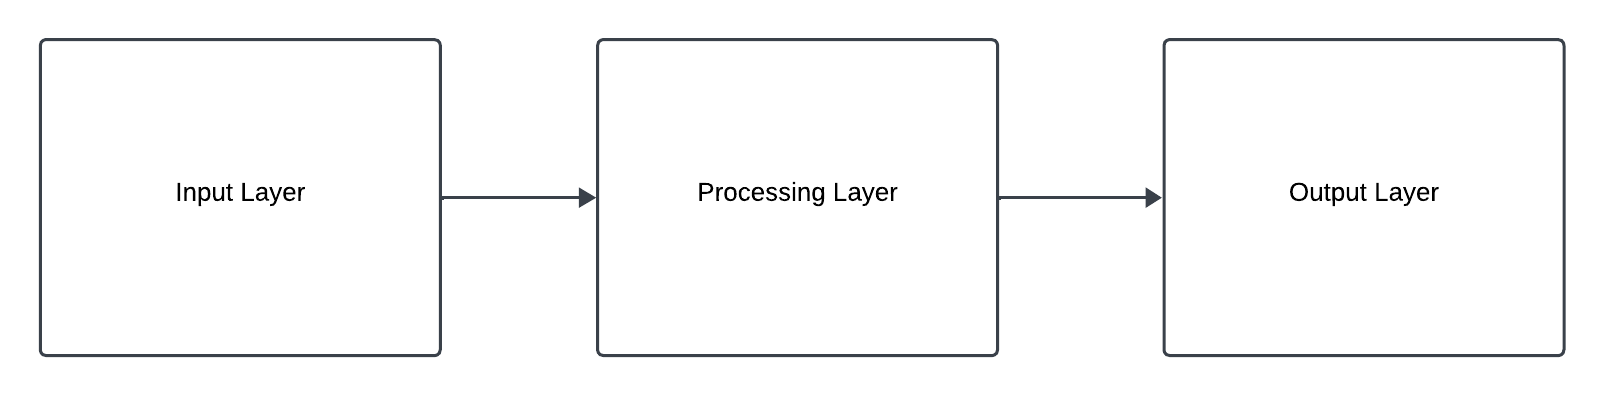
\includegraphics[width=1\textwidth]{images/sys_overview.png}
 \caption{An overview of the higher level layers.}
\end{figure}

\subsection{Input Layer Description}
The input layer plays an important part in executing the spray painting task as per the programmed movement. The input in this system comes from the host PC and the sensors. The host PC acts as a centralized location to write programs for robotic movement, as well as control PLC logic. The sensors involved in the system are emergency stops (e-stops) and inductive switches. These inputs sends signals to the PLC on particular situations and scenarios to keep the safety measure intact. Inductive switches make sure that the robot arm is calibrated properly before it executes its task. Where as emergency stops immediately halt the robot's operation, ensuring the safety of personnel and preventing potential accidents.

\subsection{Processing Layer Description}
The processing layer comprises of connection and communication between the PLC and the robot controller primarily. In order to program the PLC to do the required tasks, GXWorks3 (software) and RTToolbox (software) are jointly used. A program written in ladder logic controls the logic for the air compressor and light tower. The program inside the PLC is written from the PC and executed. The instructions are passed onto the controller and directs the robot to move its joints according to the program. 


\subsection{Output Layer Description}

The main component of output layer is the airbrush. Movement of joints and triggering air compressor enable the robot to spray paint in desired way or pattern. The PLC sends the signals to air compressor to control the air flow of the airbrush. Whereas, the robot arm adjust itself according to the programmed positions before the air brush sprays. In addition, there is a light tower which consist of 3 lights. Every color outputs different signal. Green light indicates the regular functioning of the robot. The yellow light is only visible when the robot is calibrating itself with the help of inductive switches. Red light indicates the error or e-stop status, which signals in the halt state of the robot.


